
\section{Avalanche involving a dry area}

An avalanche test problem involving a dry area. Here debris is approximated as water. The simulation should show a rarefaction fan and wetting process. 

\subsection{Results}


We should see excellent agreement between the analytical and numerical solutions.

\begin{figure}[h]
\begin{center}
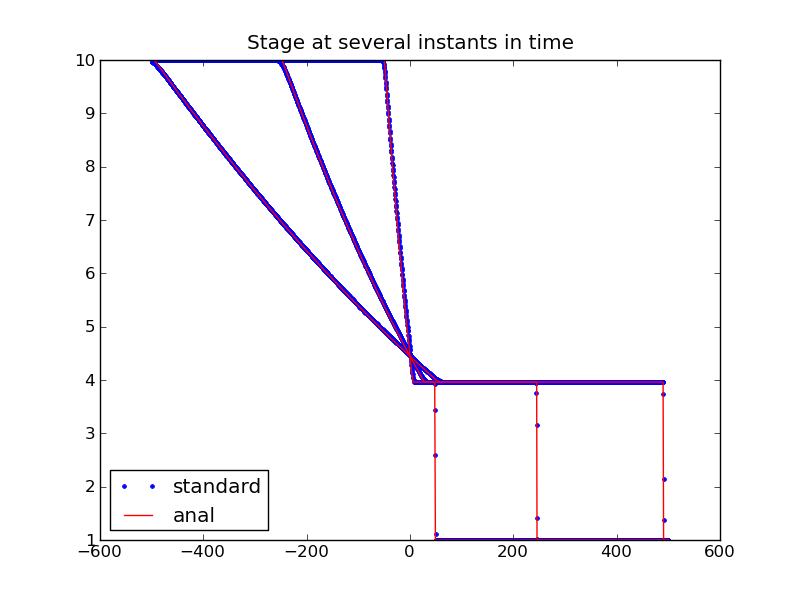
\includegraphics[width=0.9\textwidth]{stage_plot.png}
\end{center}
\caption{Stage results}
\end{figure}


\begin{figure}[h]
\begin{center}
\includegraphics[width=0.9\textwidth]{xmom_plot.png}
\end{center}
\caption{Xmomentum results}
\end{figure}


\begin{figure}[h]
\begin{center}
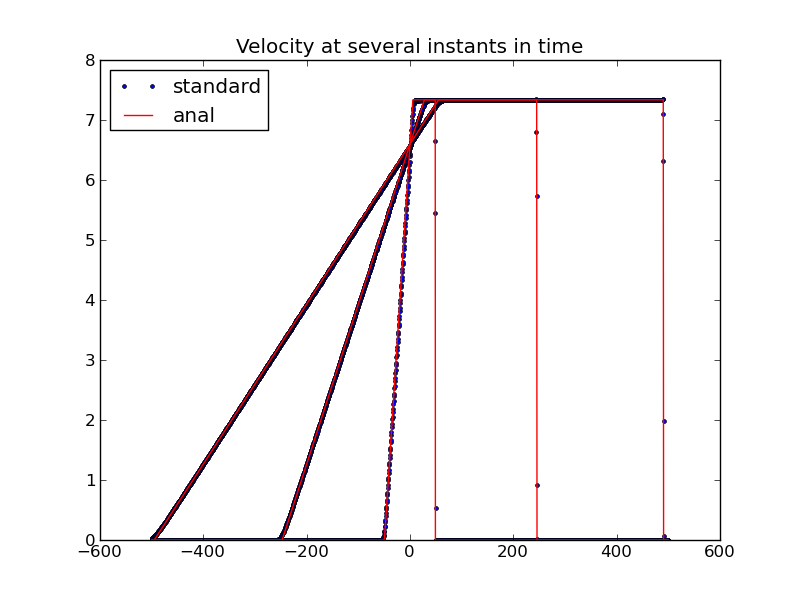
\includegraphics[width=0.9\textwidth]{xvel_plot.png}
\end{center}
\caption{Xvelocity results}
\end{figure}


\endinput
